\documentclass[t]{beamer}

%\documentclass[handout, t]{beamer}
\setbeamertemplate{navigation symbols}{}
\usepackage{pstricks}
\usepackage{mathtools}
\usepackage{amsfonts}
\usepackage{mathrsfs}
\usepackage{amsmath}
\setbeamertemplate{navigation symbols}{}
\usepackage{bm}
\usepackage[UTF8]{ctex}
\usetheme{AnnArbor}
\usefonttheme{serif}
\useinnertheme{rounded}
%\usecolortheme{crane}
\setbeamertemplate{blocks}[rounded][shadow=true]

\newcommand{\dif}{{\;\rm d}}
\usepackage{graphicx}
\usepackage{pgf}
\usepackage{tikz}
\usetikzlibrary{arrows, decorations.pathmorphing, backgrounds, positioning, fit, petri, automata}
\tikzset{>=stealth}

\usepackage{setspace}
\setmainfont{Times New Roman}
\setCJKmainfont{Microsoft YaHei}


\hypersetup{pdfpagemode=FullScreen}
\renewcommand{\Pr}{\mathbb{P}}
\usepackage{blkarray}


\setbeamercolor{block title}{bg=red!10!white}
\setbeamercolor{block body}{bg=gray!10!white}

\usepackage{multicol}
\newcommand{\E}{\mathbb{E}}
\newcommand{\EP}{\mathbb{E}^{\mathbb{P}}}
\newcommand{\EQ}{\mathbb{E}^{\mathbb{Q}}}
\newcommand{\Var}{{\rm Var}}
\newcommand{\Cov}{{\rm Cov}}


\begin{document}
\fontsize{11}{18}\selectfont


\CTEXindent



  \title{第二章~~离散时间马氏链1}
\author{随机过程及其在金融中的应用}
\date{中国人民大学出版社}
  \begin{frame}
    \maketitle
  \end{frame}

\begin{frame}{本章内容}
  \begin{multicols}{2}
    \tableofcontents
  \end{multicols}
\end{frame}

\begin{frame}{简介}
    根据状态和时间的特点,随机过程既有离散状态和连续状态,也有离散时间和连续时间。将它们加以组合,便可以得到不同类别的随机过程。

    最简单的一类随机过程便是状态和时间均离散的离散时间马氏链(discrete-time Markov chain)。该随机过程因俄国数学家安德烈·马尔可夫而得名。
    \begin{center}
        \includegraphics[height=.38\textheight]{fig/markov.jpg}
    \end{center}
\end{frame}



\section{定义和例子}

\subsection{马氏链的定义}
\begin{frame}{基本概念}
    考虑一个离散时间的随机过程$X_n\; (n=0,1,2,\ldots)$,$X_n$在有限集合$S$内取值,称$X_n$的所有可能取值为系统的状态(state),相应的集合$S$称作状态空间(state space)。

    定义转移概率(transition probability),其表达式如下:
\[
p_{n+1}(i,j)=\Pr\big(X_{n+1}=j\;|\;{X_n=i},\; X_{n-1}=i_{n-1},X_{n-2}=i_{n-2},\;\ldots,\; X_{0}=i_{0}\big)
\]
可见,转移概率$p_{n+1}(i,j)$是一个条件概率,度量的是过程$X_n$在过去$0\sim n$期状态的条件下,第$(n+1)$期状态为$j$的概率。
\end{frame}


\begin{frame}{马氏性和马氏链}
    如果$p_{n+1}(i,j)=\Pr(X_{n+1}=j\;|\;{X_n=i})$,称这个过程$X_n$具有马氏性(Markov property),相应的过程称作马氏链(Markov chain)。
    即:$X_{n+1}$的状态$j$只与$X_n$的状态$i$有关,而与之前各期的状态$i_{n-1},\ldots,i_0$无关。

    \begin{center}
    \begin{tikzpicture}[>=stealth]
        \draw[->, very thick](-4.5,0)--(4,0);
        \draw(-3,.15)--(-3,-.15);
        \draw(-1.5,.15)--(-1.5,-.15);
        \draw(0,.15)--(0,-.15);
        \draw(1.5,.15)--(1.5,-.15);
        \draw(3,.15)--(3,-.15);
        \draw (-3,-.5) node  {$X_{n-2}$};
        \draw (-1.5,-.5) node  {$X_{n-1}$};
        \draw (0,-.5) node  {$X_{n}$};
        \draw (1.5,-.5) node  {$X_{n+1}$};
        \draw (3,-.5) node  {$X_{n+2}$};
        \draw (-4,-.5) node  {$\cdots$};
        
        \draw (0,.5) node  {现在};
        \draw (1.5,.5) node  {将来};
        \draw (3,.5) node  {$\to$};
        \draw (-2.5,.5) node  {$\leftarrow$};
        \draw (-1.5,.5) node  {过去};
        \end{tikzpicture}
\end{center}
    
马氏性可以通俗地表述为:已知{“现在”$X_n$} 的条件下,{“将来”$X_{n+1}$} 与{“过去”($X_{n-1},\ldots,X_1,X_0$)} 无关的特性。
\end{frame}


\begin{frame}{马氏性和马氏链(cont.)}
    \begin{center}
        \begin{tikzpicture}[>=stealth]
            \draw[->, very thick](-4.5,0)--(4,0);
            \draw(-3,.15)--(-3,-.15);
            \draw(-1.5,.15)--(-1.5,-.15);
            \draw(0,.15)--(0,-.15);
            \draw(1.5,.15)--(1.5,-.15);
            \draw(3,.15)--(3,-.15);
            \draw (-3,-.5) node  {$X_{n-2}$};
            \draw (-1.5,-.5) node  {$X_{n-1}$};
            \draw (0,-.5) node  {$X_{n}$};
            \draw (1.5,-.5) node  {$X_{n+1}$};
            \draw (3,-.5) node  {$X_{n+2}$};
            \draw (-4,-.5) node  {$\cdots$};
            
            \draw (0,.5) node  {现在};
            \draw (1.5,.5) node  {将来};
            \draw (3,.5) node  {$\to$};
            \draw (-2.5,.5) node  {$\leftarrow$};
            \draw (-1.5,.5) node  {过去};
            \end{tikzpicture}
    \end{center}

    $X_{n+1}$的状态只与$X_n$的状态有关;$X_{n}$的状态只与$X_{n-1}$的状态有关;……,各期状态只与其前一期的状态有关,如此环环相扣,如同锁链一般,这也是该过程得名“马氏链”的原因。

    更进一步,如果假设时刻$n$的取值与转移概率无关,即:
\begin{equation*}
\Pr(X_{n+1}=j\;|\;{X_n=i})=p(i,j),\qquad \forall n
\end{equation*}
则该性质称为时间齐次性(time-homogeneous),简称“时齐”。相应的马氏链称作时齐马氏链。
\end{frame}

\subsection{马氏链的例子}
\begin{frame}{举例1:赌徒破产问题}
    \normalsize
    赌徒在一次赌博中,赢得1元的概率是0.4;输掉1元的概率是0.6。
    赌徒退出赌博的条件为:输光(财富为零),或者财富数额达到$N$元。
    
    假设随机变量$X_{n}$表示赌徒在第$n$次赌博后的财富数量。可见,
    $X_{n+1}$只与$X_n$有关,而与之前的状态($X_{n-1},\ldots,X_0$)无关,$X_n$具有{马氏性},即:
    \[\begin{split}
    \Pr(X_{n+1}&=j\;|\;{X_n=i}, X_{n-1}=i_{n-1}, X_{n-2}=i_{n-2},\ldots, X_{0}=i_{0})\\&=\Pr(X_{n+1}=j\;|\;{X_n=i})=p(i,j)
    \end{split}\]

    这里的$p(i,j)$就是转移概率。对于赌徒而言,其第$(n+1)$次赌博输赢的条件概率为:
\[\begin{split}
p(i,i-1)=\Pr(X_{n+1}=i-1\;|\;X_n=i)&=0.6,\qquad \text{输}\\
p(i,i+1)=\Pr(X_{n+1}=i+1\;|\;X_n=i)&=0.4,\qquad \text{赢}
\end{split}\]
\end{frame}

\begin{frame}{转移概率矩阵}
    此处$p(i,j)$的相应数值,可以标注在一个矩阵的第$i$行、第$j$列。这样的矩阵{\bf P}称为{转移概率矩阵}(transition matrix)。
    \[{\bf P}=\begin{bmatrix}
    p(0,0)& p(0,1)& \cdots &p(0,N)\\
    p(1,0)& p(1,1)&\cdots &p(1,N)\\
    \vdots &\vdots &\ddots &\vdots \\
    p(N,0)& p(N,1)&\cdots &p(N,N)\\
    \end{bmatrix}\]
\end{frame}

\begin{frame}{转移概率矩阵(cont.)}
    当$N=5$时,转移概率矩阵如下:
    \begin{center}
    ${\bf P}=$\begin{blockarray}{ccccccc}
    & 0 & 1 & 2 & 3 & 4 & 5\\
    \begin{block}{c[cccccc]}
    0 & 1 & 0 & 0 & 0 & 0 & 0\\
    1 & 0.6 & 0 & 0.4 & 0 & 0 & 0\\
    2 & 0 & 0.6 & 0 & 0.4 & 0 & 0\\
    3 & 0 & 0 & 0.6 & 0 & 0.4 & 0\\
    4 & 0 & 0 & 0 & 0.6 & 0 & 0.4\\
    5 & 0 & 0 & 0 & 0 & 0 & 1\\
    \end{block}
    \end{blockarray}
    \end{center}

    在该问题中,马氏链的状态空间$S=\{0,1,2,3,4,5\}$,这是一个有限状态的马氏链。
\end{frame}


\begin{frame}{转移概率图}
    根据该马氏链的状态及各状态之间的转移概率,还可以绘制出相对应的转移概率图。
    \begin{figure}
    \centering
    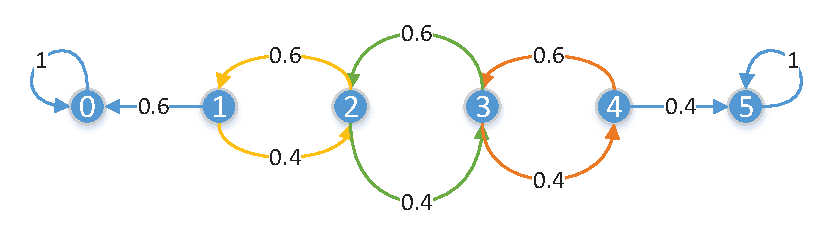
\includegraphics[scale=0.7]{fig/markov11.eps}
    \end{figure}

    在该问题中,$p(0,0)=1, \; p(5,5)=1$。这意味着当前时刻到达状态0或5时,下一时刻将仍然停留在原来的状态。在赌徒破产问题中,这意味着赌徒最终破产或赢钱离开,其财富数量不再发生变化。这样的状态(0和5)称为吸收态(absorbing state)。
\end{frame}


\begin{frame}{举例2:埃伦费斯特链(Ehrenfest Chain)}
    总共有$N$个球,且这些球只可能在罐子A或B中。每次随机地从任一罐子中取球一个,并投入另一罐子中。
	
    假设$n$时刻罐子A中有$i$个球,则:
    \begin{enumerate}
    \item $(n+1)$时刻罐子A中有$(i+1)$个球的概率是$(N-i)/N$;
    \item $(n+1)$时刻罐子A中有$(i-1)$个球的概率是$i/N$。
    \end{enumerate}
    即:\[p(i,i+1)=\frac{N-i}{N},\quad p(i,i-1)=\frac{i}{N}\qquad 1\le i\le N-1\]
    另外,$p(0,1)=1,\; p(N,N-1)=1$ 分别表示当罐子A中没有球时,下一次只可能从罐子B中取球放入罐子A中;类似地,当罐子A中球满时,下一次只可能从罐子A中取球放入罐子B中。
\end{frame}


\begin{frame}{埃伦费斯特链(cont.)}
    当球的数量$N=4$时,可以得到对应的转移概率矩阵如下:
	\begin{center}
${\bf P}=$\begin{blockarray}{cccccc}
 & 0 & 1 & 2 & 3 & 4 \\
 \begin{block}{c[ccccc]}
 0 & 0 & 1 & 0 & 0 & 0 \\
1 & 0.25 & 0 & 0.75 & 0 & 0 \\
2 & 0 & 0.5 & 0 & 0.5 & 0 \\
3 & 0 & 0 & 0.75 & 0 & 0.25 \\
4 & 0 & 0 & 0 & 1 & 0  \\
\end{block}
\end{blockarray}
\end{center}
\end{frame}


\begin{frame}{马氏链的转移概率性质}
\begin{itemize}
    \item $p(i,j)\ge 0$,转移概率非负;

    \item $\displaystyle\sum_j p(i,j)=1$,转移概率矩阵每行元素之和均为1。可以看出,转移概率矩阵${\bf P}$每行元素之和一定等于1,因为从一个状态转移到其余所有可能状态的概率之和必须满足概率的完备性。
\end{itemize}
\end{frame}

\begin{frame}{举例3:库存链}
    假设有一个电子产品店,若一天结束时,某款游戏的库存量为1或0,则他们需要订购足够单位的商品,以使得第二天开始时的库存总量为5。假设第二天的需求数量$k$及对应的概率如下:
    \begin{center}
    \begin{tabular}{c|cccc}
    \hline
    $k$ &0 &1& 2& 3\\
    \hline
    $\Pr$&0.3&0.4&0.2&0.1\\
    \hline
    \end{tabular}
    \end{center}
    求库存链的转移概率矩阵。
\end{frame}

\begin{frame}{库存链(cont.)}
    在该问题中,我们关注的是电子产品店一天结束时游戏的库存量,其状态空间为:$S=\{0,1,2,3,4,5\}$ (因为库存总量不超过5)。

    \begin{center}
        ${\bf P}=$\begin{blockarray}{ccccccc}
         & 0 & 1 & 2 & 3 & 4 &5\\
         \begin{block}{c[cccccc]}
         0 & 0 & 0 & 0.1 & 0.2 & 0.4 &0.3\\
        1 & 0 & 0 & 0.1 & 0.2 & 0.4 &0.3 \\
        2 & 0.3 & 0.4 & 0.3 & 0 & 0 &0\\
        3 & 0.1 & 0.2 & 0.4 &0.3& 0 &0\\
        4 & 0 & 0.1 & 0.2 & 0.4 &0.3  &0\\
        5 & 0 & 0 & 0.1 & 0.2 & 0.4 &0.3\\
        \end{block}
        \end{blockarray}
        \end{center}
\end{frame}



\begin{frame}{举例4:修复链}
    一台机器有三个关键零件容易出故障,但只要其中两个能工作,机器就可正常运行。当有两个出故障时,它们将被替换,并于第二天恢复正常运转,以损坏的零件
    序号$\{0,1,2,3,12,13,23\}$为状态空间,并假定没有两个零件在同一天损坏,且三个零件损坏的概率分别为:
    \begin{center}
        \begin{tabular}{c|ccc}
        \hline
        序号  &1& 2& 3\\
        \hline
        $\Pr$&0.01&0.02&0.04\\
        \hline
        \end{tabular}
        \end{center}
\end{frame}


\begin{frame}{修复链(cont.)}
    修复链的转移概率矩阵如下:
	\begin{center}
${\bf P}=$\begin{blockarray}{ccccccccc}
 & 0 & 1 & 2 & 3 & 12 &13 &23\\
 \begin{block}{c[cccccccc]}
 0 & 0.93& 0.01 & 0.02 & 0.04 & 0 &0&0\\
1 & 0 & 0.94 & 0 & 0 & 0.02 &0.04&0 \\
2 & 0 & 0 & 0.95 & 0 & 0.01 &0&0.04\\
3 & 0 & 0 & 0 &0.97& 0 &0.01&0.02\\
12 & 1 & 0 & 0 & 0 &0  &0 &0\\
13 & 1 & 0 & 0 & 0 &0  &0 &0\\
23 & 1 & 0 & 0 & 0 &0  &0 &0\\
\end{block}
\end{blockarray}
\end{center}
\end{frame}

\section{多步转移概率}
\begin{frame}{多步转移概率}
    $p(i,j)=\Pr(X_{n+1}=j\;|\;X_{n}=i)$给出了从状态$i$到$j$的一步转移概率;类似地,从$i$到$j$的$m$步($m>1$)转移概率定义为:
    \begin{equation*}
    p^m(i,j)=\Pr(X_{n+m}=j\;|\;X_{n}=i)
    \end{equation*} 
    这里的$p^m(i,j)$是$m$步转移概率矩阵${\bf P}^m$第$i$行、第$j$列的数值。

    \begin{block}{定理:}
        $m$步转移概率矩阵是1步转移概率矩阵${\bf P}$的$m$次幂,即${\bf P}^m$。
    \end{block}
\end{frame}

\subsection{多步转移概率的求解}
\begin{frame}{多步转移概率的求解}


以两步转移概率为例:假定状态总数为$n$,初始状态为$X_0=i$,经过一步转移状态变为$X_1=k, \;k=1,2,\ldots,n$,最终的状态为$X_2=j$,求$p^2(i,j)$。
\[i\longrightarrow k\longrightarrow j\]
由于$$p^2(i,j)=\Pr(X_2=j\;|\;X_0=i)=\sum_{k=1}^{n}\Pr(X_2=j,X_1=k\;|\;X_0=i) $$
\end{frame}

\begin{frame}{多步转移概率的求解(cont.)}
对$\Pr(X_2=j,X_1=k\;|\;X_0=i)$进行展开,可得:
\[\begin{split}
\Pr(X_2=j,X_1=k\;|\;X_0=i)&=\frac{\Pr(X_2=j,X_1=k,X_0=i)}{\Pr(X_0=i)}\\
&=\frac{\Pr(X_2=j,X_1=k,X_0=i)}{\Pr(X_1=k,X_0=i)}\cdot \frac{\Pr(X_1=k,X_0=i)}{\Pr(X_0=i)}\\
&={\Pr(X_2=j\;|\;X_1=k,X_0=i)}\cdot \Pr(X_1=k\;|\;X_0=i)
\end{split}\]
根据马氏性,$\Pr(X_2=j\;|\;X_1=k,X_0=i)=\Pr(X_2=j\;|\;X_1=k)$,因此:
\[\text{上式}=\Pr(X_1=k\;|\;X_0=i)\cdot {\Pr(X_2=j\;|\;X_1=k)}=p(i,k)\cdot {p(k,j)} \]
最终:
\[
p^2(i,j)=\Pr(X_2=j\;|\;X_0=i)=\sum_{k=1}^{n} p(i,k)\cdot p(k,j)
\]
\end{frame}

\begin{frame}{多步转移概率的求解(cont.)}
    将方程$p^2(i,j)=\displaystyle\sum_{k=1}^{n} p(i,k)\cdot p(k,j)$使用矩阵表示如下:
    \begin{equation*}\scriptsize
    \underbrace{\begin{bmatrix}
        p(1,1)&p(1,2)&\cdots &p(1,n)\\
        p(2,1)&p(2,2)&\cdots &p(2,n)\\
        \vdots&\vdots&\ddots&\vdots\\
        \boxed{p(i,1)}& \boxed{p(i,2)}&\cdots &\boxed{p(i,n)}\\
        \vdots&\vdots&\ddots&\vdots\\
        p(n,1)& p(n,2)&\cdots &p(n,n)\\
        \end{bmatrix}}_{\bf P}\underbrace{\begin{bmatrix}
        p(1,1)&p(1,2)&\cdots &\boxed{ p(1,j)}&\cdots&p(1,n)\\
        p(2,1)&p(2,2)&\cdots &\boxed{ p(2,j)}&\cdots&p(2,n)\\
        \vdots&\vdots& \ddots&\vdots&\ddots&\vdots\\
        p(n,1)&p(n,2)&\cdots &\boxed{ p(n,j)}&\cdots&p(n,n)\\
        \end{bmatrix}}_{\bf P} 
    \end{equation*}
        可见,$p^2(i,j)$是转移概率矩阵二次幂${\bf P}^2$第$i$行、第$j$列的数值。相应的${\bf P}^2$表示两步转移的转移概率矩阵。
\end{frame}

\subsection{多步转移概率举例}
\begin{frame}{赌徒破产问题回顾}
    在赌徒破产问题中,一步转移概率矩阵如下:
    \begin{equation*}
    {\bf P}=\begin{bmatrix}
     1 & 0 & 0 & 0 & 0 & 0\\
     0.6 & 0 & 0.4 & 0 & 0 & 0\\
     0 & 0.6 & 0 & 0.4 & 0 & 0\\
     0 & 0 & 0.6 & 0 & 0.4 & 0\\
     0 & 0 & 0 & 0.6 & 0 & 0.4\\
     0 & 0 & 0 & 0 & 0 & 1\\
    \end{bmatrix}
    \end{equation*}
    相应地,如果要求解$n$步的转移概率矩阵${\bf P}^n$,只需对${\bf P}$取$n$次幂即可。
\end{frame}


\begin{frame}{1000步的转移概率矩阵}
    我们可以用软件算出1000步赌博后的转移概率矩阵,最终的结果如下:
    \begin{equation*}
        {\bf P}^{1000}=\begin{bmatrix}  
            1     &    0   &      0   &      0    &     0  &       0\\
            0.9242  &  0   &      0  &  0  &      0  &  0.0758\\
            0.8104  &       0 &   0  &       0  &  0  &  0.1896\\
            0.6398  &  0      &   0  &  0  &      0  &  0.3602\\
            0.3839   &      0  &  0  &      0  &  0   & 0.6161\\
                 0  &       0  &       0  &       0    &     0 &   1\\
        \end{bmatrix} 
        \end{equation*} 

        随着赌徒不断地进行赌博,其最终的结果只有两个:破产或获利出局。
赌徒在入局之时,如果只有1元,其最终破产的概率高达92.42\%;如果有4元,其最终破产的概率也高达38.39\%。
\end{frame}


\begin{frame}{库存链回顾}
    对于库存链,可以使用软件算出其在$1000$步的转移概率矩阵,最终的结果如下:
    \[{\bf P}^{1000}=\begin{bmatrix}
        0.0909 & 0.1556 & 0.2310 & 0.2156 & 0.2012 & 0.1056\\
        0.0909 & 0.1556 & 0.2310 & 0.2156 & 0.2012 & 0.1056\\
        0.0909 & 0.1556 & 0.2310 & 0.2156 & 0.2012 & 0.1056\\
        0.0909 & 0.1556 & 0.2310 & 0.2156 & 0.2012 & 0.1056\\
        0.0909 & 0.1556 & 0.2310 & 0.2156 & 0.2012 & 0.1056\\
        0.0909 & 0.1556 & 0.2310 & 0.2156 & 0.2012 & 0.1056\\
        \end{bmatrix}\]

        这样的转移概率矩阵每列的数值均相同。这说明从任意状态$x$,经过1000步转移到某个状态$y$的概率均相等。
\end{frame}


\begin{frame}{埃伦费斯特链回顾}
    ${\bf P}^{1000}={\bf P}^{1002}$,但是${\bf P}^{1000}\ne {\bf P}^{1001}$。如果继续计算第1003步甚至更多步,会发现最终转移概率矩阵呈现出${\bf P}^{1000}$和${\bf P}^{1001}$的结果交替出现的现象,这被称为马氏链的周期性(periodicity)。
\end{frame}

\subsection{C-K方程}
\begin{frame}{查普曼-柯尔莫哥洛夫(Chapman-Kolmogorov, C-K)方程}
        \begin{figure}[htp]
            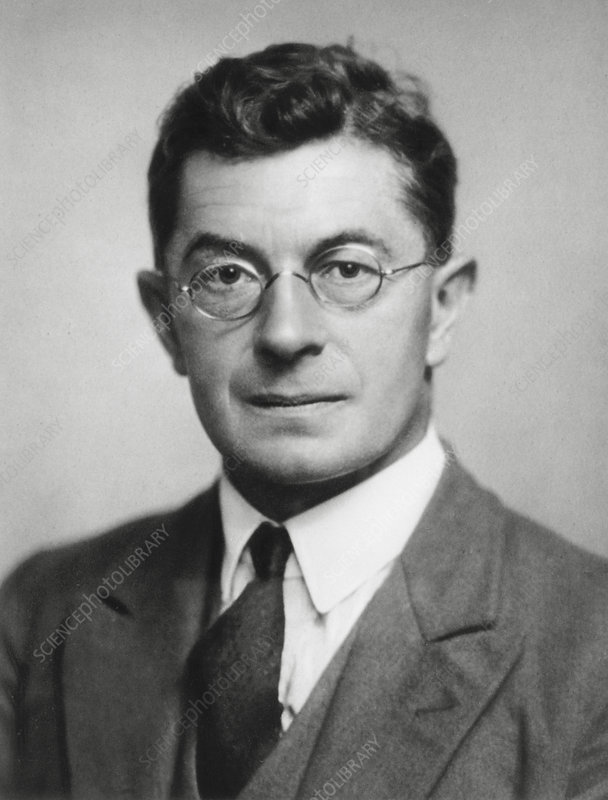
\includegraphics[height=.4\textheight]{fig/chapman.jpg}
            \quad 
            \includegraphics[height=.4\textheight]{fig/kolmogorov.jpg}
            \centering
            \end{figure}
            \begin{equation*}
                p^{m+n}(i,j)=\Pr(X_{m+n}=j\;|\;X_0=i)=\sum_k p^m(i,k)\cdot p^n(k,j)
                \end{equation*}
        
\end{frame}

\begin{frame}{C-K方程的简要证明}
    \small
    由于$$p^{m+n}(i,j)=\Pr(X_{m+n}=j\;|\;X_0=i)=\sum_k\Pr(X_{m+n}=j,X_m=k\;|\;X_0=i)$$
    其中:
    \[\begin{split}
    \Pr&(X_{m+n}=j,X_m=k\;|\;X_0=i)=\frac{\Pr(X_{m+n}=j,X_m=k,X_0=i)}{\Pr(X_0=i)}\\
    &=\frac{\Pr(X_{m+n}=j,X_m=k,X_0=i)}{\Pr(X_m=k,X_0=i)}\cdot \frac{\Pr(X_m=k,X_0=i)}{\Pr(X_0=i)}\\
    &={\Pr(X_{m+n}=j\;|\;X_m=k,X_0=i)}\cdot \Pr(X_m=k\;|\;X_0=i)\\
    &={\Pr(X_{m+n}=j\;|\;X_m=k)}\cdot \Pr(X_m=k\;|\;X_0=i)\\
    &={p^n(k,j)}\cdot p^m(i,k)\\
    \end{split}\]
    因此:$$p^{m+n}(i,j)=\sum_k p^m(i,k)\cdot p^n(k,j)$$
\end{frame}

\begin{frame}{C-K方程的推论}
\begin{block}{C-K方程}
    \begin{equation*}
        p^{m+n}(i,j)=\sum_k p^m(i,k)\cdot p^n(k,j)
        \end{equation*}
\end{block}

    由于$\forall k$,$p^m(i,k)\cdot p^n(k,j)\ge 0$,因此基于C-K方程,还能得到如下不等式:
    \begin{equation*}
    p^{m+n}(i,j)\ge  p^m(i,k)\cdot p^n(k,j) ,\qquad \forall k
    \end{equation*}
\end{frame}

\section{状态的分类}
\begin{frame}{状态分类的意义}
    我们研究马氏链,主要是进行两类分析:瞬态分析和稳态分析。
\begin{itemize}
    \item 瞬态分析是研究在某一固定时刻$n$,马氏链对应系统的概率特征,即求$n$步转移概率。
    \item 稳态分析则是研究当$n\to\infty$时,马氏链对应系统的概率特征,比如:$\lim\limits_{n\to\infty}p^n(i,j)$是否存在;与状态的关系如何;极限概率能否构成概率分布。
\end{itemize}
    
    为解决这两类问题,就需要对状态进行分类。
\end{frame}


\begin{frame}{几个重要的标记}
    \begin{itemize}
        \item 初始时刻状态为$x$的条件下,事件A发生的概率记作$\Pr_x(A)$,即:
        \begin{equation*}
        \Pr_x(A)=\Pr(A|X_0=x)
        \end{equation*}
        
        \item 首次返回状态$x$的最短时间记作$\tau_x$,即:
        \begin{equation*}
        \tau_x=\min\{n: n\ge 1, X_n=x \}
        \end{equation*}
        需要注意的是,随机过程随不同的路径演化,相应的首次返回的时间也是随机变动的,因此$\tau_x$是随机的。
        
        \item  第$k$次返回状态$x$的最短时间记作$\tau^k_x$,即:
        \begin{equation*}
        \tau^k_x=\min\left\{n:n>\tau^{k-1}_x, X_n=x \right\}
        \end{equation*}
    \end{itemize}

    \end{frame}


    \begin{frame}{几个重要的标记(cont.)}
        \begin{itemize} 
        \item  从初始时刻的状态$x$,经过有限步{首次返回}到状态$x$的概率记作$f_{xx}$,即:
        \begin{equation*}
        f_{xx}=\Pr_x(\tau_x<\infty)=\Pr(\text{有限时间首次返回$x$状态}|X_0=x)
        \end{equation*}
        由于当$n=0$时,$f_{xx}\equiv 1$,因此为避免该情况,规定$n\ge 1$。
        
        \item  经过有限时间,返回状态$x$的次数为$k$的概率记作$f_{xx}^{\,k}$,即:
        \begin{equation*}
        f_{xx}^{\,k}=\Pr_x(\tau^k_x<\infty)=\Pr(\text{有限时间第$k$次返回$x$状态}|X_0=x)
        \end{equation*}
    \end{itemize}
    
    \begin{block}{注意:}
       根据后面所介绍的强马氏性,可得: $f^{\,k}_{xx}=(f_{xx})^k$
    \end{block}
\end{frame}

\subsection{停时和强马氏性}
\begin{frame}{停时的含义}
    当某事件“在时刻$n$停止”,则记该时刻$n$为停时(stopping time)。
    前面提及的首次返回状态$x$的最短时间$\tau_x$就是一个停时,可以表示为:
    \[\{\tau_x=n \}=\{X_n=x,\; X_{n-1}\ne x,\ldots,\; X_1\ne x \} \]	

    在金融市场上,经常会遇到所谓的停时概念:
    \begin{itemize}
        \item 股票价格达到一定的数值时就进行买卖操作,相应的买卖时点就可以看作一个停时;
     \item   在保险中,投保人在保险期内第一次出险,则出险的时间也可以看作一个停时;
     \item   对于美式期权,在到期前若行权能够获得收益,则该期权的买方会选择将该期权提前行权了结,那么行权的时点也是一个停时。
    \end{itemize}
    
\end{frame}


\begin{frame}{强马氏性}
    若设$T$是停时,假定$T=n$,$X_T=y$,则关于$X_0,\ldots,X_T$的其他信息与未来的预测无关,并且$X_{T+k},\; k\ge0$的行为与初始状态为$y$的马氏链相同,即:
    \[\begin{split}
    \Pr(X_{T+1}=z\;|\;X_T=y,T=n)&=\Pr(X_1=z\;|\;X_0=y)=p(y,z)\\
    \Pr(X_{T+k}=z\;|\;X_T=y,T=n)&=\Pr(X_k=z\;|\;X_0=y)=p^k(y,z),\quad k\ge 1 
    \end{split}
    \]	
    则称过程$X_T$具有强马氏性(strong Markov property)。
\end{frame}

\begin{frame}{强马氏性(cont.)}
    \begin{itemize}
        \item 马氏性是指:已知“现在”$X_n$ 的条件下,“将来”$X_{n+1}$ 与“过去”($X_{n-1},\ldots,X_1,X_0$) 无关的特性。
        \item 强马氏性则是指:已知停时$T$的条件下,将来时刻$T+1$的状态$X_{T+1}$与过去各时刻的状态无关。这两个性质的最大差别在于:马氏性当中的当前时间是确定的;而强马氏性当中的停时则是随机的。
    \end{itemize}
    

    \begin{center}
        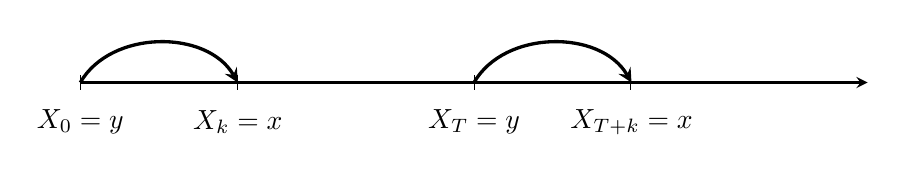
\begin{tikzpicture}[>=stealth]
            \draw[->, thick](0,0)--(10,0);
            \draw[|-|](0,0)--(2,0);
            \draw[|-|](5,0)--(7,0);
            \draw[->, very thick] (0,0) [bend left=60] to (2,0);
            \draw[->, very thick] (5,0) [bend left=60] to (7,0);
            \node at (0,-.5){$X_0=y$};
            \node at (2,-.5){$X_k=x$};
            \node at (5,-.5){$X_T=y$};
            \node at (7,-.5){$X_{T+k}=x$};
            \end{tikzpicture}
    \end{center}
\end{frame}

\subsection{可达和互通}
\begin{frame}{可达的含义}
    如果从状态$x$有正的概率到达状态$y$,则称$x$可达(accessible)$y$,记作$x\to y$,即:
	\[f_{xy}=\Pr_x(\tau_y<\infty)>0 \]
也可以表示为:
\[\exists n,\quad p^n(x,y)>0\]
即:从状态$x$,经过$n$步到达状态$y$的概率为正。


如果从状态$x$不能到达状态$y$,则记为$x\not\to y$,意味着对任意$n$,$p^n(x,y)\equiv 0$。

\end{frame}


\begin{frame}{互通的含义}
    若$x$可达$y$,并且$y$可达$x$,则称$x$和$y$互通(communicate),记作$x\leftrightarrow y$,即:
	\[x\to y,\; y\to x\quad\Rightarrow\quad  x\leftrightarrow y\]
也可以表示为:
\[\exists m,n,\quad p^m(x,y)>0,\;p^n(y,x)>0 \quad\Rightarrow\quad  x\leftrightarrow y\]
即:从状态$x$经过$m$步到达状态$y$的概率为正,并且从状态$y$经过$n$步到达状态$x$的概率也为正。
\end{frame}


\begin{frame}{互通的性质}
    互通满足自反性、对称性和传递性,即:
    \begin{enumerate}
    \item 自反性(reflexive):$x\leftrightarrow x$。
    \item 对称性(symmetric):若$x\leftrightarrow y$,则$y\leftrightarrow x$。
    \item 传递性(transitive):若$x\leftrightarrow k$,且$k\leftrightarrow y$,则$x\leftrightarrow y$。
    \end{enumerate}
\end{frame}

\subsection{状态的常返性判定}
\begin{frame}{常返态}
    若对于状态$x$,其经过有限时间可以概率1返回状态$x$,则称其为常返态(recurrent state),即:
    \[f_{xx}=\Pr_x(\tau_x<\infty)=1 \]
\begin{itemize}
    \item 当$f_{xx}=1$时,对任意$k>1$,$f_{xx}^{\, k}=1$。这意味着对于常返态$x$,其回到状态$x$的次数有无穷多次。
    \item 如果$p(x,x)=1$,即$\Pr_x(\tau_x=1)=1$,则$x$是吸收态,此时的状态$x$是非常强的常返态,因为马氏链的状态将永远停留在那里。
\end{itemize}
    \end{frame}


\begin{frame}{非常返态}
    若对于状态$x$,其经过有限时间有正的概率不再返回状态$x$,则称其为非常返态(transient state),也称暂态,即:
    \[\Pr_x(\tau_x=\infty)>0\]
    或者\[f_{xx}=\Pr_x(\tau_x<\infty)=1-\Pr_x(\tau_x=\infty)<1 \]

    根据强马氏性,当$f_{xx}<1$时,随着$k\to\infty$,$f_{xx}^{\, k}\to 0$,这意味着最终马氏链将不再回到状态$x$。
\end{frame}

\begin{frame}{等价表达式}
    \begin{enumerate}
        \item 常返:状态$x$在有限时间内(首次)返回$x$的概率为1。
        \[f_{xx}=1  \quad\Longleftrightarrow\quad  \Pr_{x}(\tau_x<\infty)=1  \quad\Longleftrightarrow\quad   \Pr_{x}(\tau_x=\infty)=0\]
        \item 非常返:状态$x$有正的概率不返回$x$。
        \[f_{xx}<1  \quad\Longleftrightarrow\quad  \Pr_{x}(\tau_x<\infty)<1  \quad\Longleftrightarrow\quad   \Pr_{x}(\tau_x=\infty)>0\]  
        \end{enumerate}
        
\end{frame}

\begin{frame}{定理}
    若记$\E_x[N(y)]$是在初始状态为$x$的条件下,访问状态$y$的次数之期望值,则:
    \[\E_x[N(y)]=\frac{f_{xy}}{1-f_{yy}}=\sum^{\infty}_{n=1} p^n(x,y) \]
\end{frame}



\begin{frame}{证明$\E_x[N(y)]=\frac{f_{xy}}{1-f_{yy}}$(方法一)}
    由于$N(y)$是访问状态$y$的次数,因此从状态$x$开始访问状态$y$的次数为$k$的概率为:
    \[\begin{split}
    \Pr_x[N(y)=k]&=\Pr_{x}(\tau_y^k <\infty)\cdot \Pr_{y}(\tau_y^{k+1} =\infty) \\
    &=f_{xy}\cdot f_{yy}^{k-1} \cdot (1-f_{yy})
    \end{split}
    \]

    根据期望的定义得到:
\[\begin{split}
\E_x[N(y)]&= \sum_{k=1}^{\infty} k\cdot \Pr_x[N(y)=k]= \sum_{k=1}^{\infty} k\cdot \left[f_{xy}\cdot f_{yy}^{\;k-1} \cdot (1-f_{yy})\right]\\
&= f_{xy}(1-f_{yy}) \sum_{k=1}^{\infty} k\cdot f_{yy}^{\;k-1}  \\
&= f_{xy}(1-f_{yy}) \cdot \frac{1}{(1-f_{yy})^2}=\frac{f_{xy}}{1-f_{yy}}
\end{split} \]
\end{frame}


\begin{frame}{证明$\E_x[N(y)]=\frac{f_{xy}}{1-f_{yy}}$(方法二)}
   由于 \[\E_x[N(y)]=\sum_{k=1}^{\infty} \Pr_x[N(y)\ge k] \]
    其中:
    \[\begin{split}
    \Pr_x[N(y)\ge k]&=\sum^{\infty}_{n=k} \Pr_x[N(y)=n]=\sum^{\infty}_{n=k} f_{xy}f^{\;n-1}_{yy}(1-f_{yy})\\
    &=f_{xy}(1-f_{yy})\sum^{\infty}_{n=k} f^{\;n-1}_{yy}=f_{xy}(1-f_{yy})\cdot \frac{f^{\;k-1}_{yy}}{1-f_{yy}}\\
    &=f_{xy}\cdot f^{\;k-1}_{yy}
    \end{split}\]
    因此:
    \[\E_x[N(y)]=\sum_{k=1}^{\infty}f_{xy}\cdot f^{\;k-1}_{yy}=\frac{f_{xy}}{1-f_{yy}}  \]
\end{frame}


\begin{frame}{证明
    $\E_x[N(y)]=\sum^{\infty}_{n=1} p^n(x,y)$}
    根据示性函数(indicator function)的性质
    \[N(y)=\sum_{n=1}^{\infty}{\bf 1}_{\{X_n=y\}} \]
    对上式两端求条件期望,可得:
    \[\E_x[ N(y)]=\sum_{n=1}^{\infty}\Pr_{x}(X_n=y)=\sum_{n=1}^{\infty} p^n(x,y)\]
\end{frame}


\begin{frame}{$\E_x[N(y)]=\frac{f_{xy}}{1-f_{yy}}=\sum^{\infty}_{n=1} p^n(x,y)$}
    \begin{itemize}
        \item  若状态$y$是常返态,则意味着$f_{yy}=1$,此时可得:$\E_x[N(y)]=\infty$。因此,对于常返态$y$而言,其访问状态$y$的次数的期望值为无穷大;同时,$\displaystyle\sum^{\infty}_{n=1} p^n(x,y)=\infty$。
        \item 若状态$y$是非常返态,则意味着$f_{yy}<1$,相应地,$\E_x[N(y)]<\infty$,对应的$\displaystyle\sum^{\infty}_{n=1} p^n(x,y)<\infty$。
    \end{itemize}
   

    
\end{frame}

\begin{frame}{等价表达式}
    \begin{enumerate}
        \item 常返态:从状态$x$无限次返回$x$。
        \[f_{xx}=1   \quad\Longleftrightarrow\quad   \E_x[N(x)]=\infty \quad\Longleftrightarrow\quad  \sum^{\infty}_{n=1} p^n(x,x)=\infty \] 
        \item 非常返态:从状态$x$有限次返回$x$。
        \[f_{xx}<1   \quad\Longleftrightarrow\quad   \E_x[N(x)]<\infty \quad\Longleftrightarrow\quad \sum^{\infty}_{n=1} p^n(x,x)<\infty \] 
        \end{enumerate}
\end{frame}

\begin{frame}{若干定理}
\begin{itemize}
    \item 若状态$x$是常返态,并且$x\to y$,则状态$y$是常返态。
    \item 若$f_{xy}>0$,且$f_{yx}<1$,则$x$是非常返态。
    \item 若状态$x$是常返态,并且$f_{xy}>0$,则$f_{yx}=1$。
\end{itemize}
\end{frame}


\begin{frame}{举例5:七状态马氏链}
    考虑如下转移概率矩阵:
    \begin{center}
    ${\bf P}=$\begin{blockarray}{cccccccc}
        &1 & 2 &3 & 4&5 &6 &7 \\	
        \begin{block}{c[ccccccc]}
    1&0.7&0&0&0&0.3&0&0\\
    2&0.1&0.2&0.3&0.4&0&0&0\\
    3&0&0&0.5&0.3&0.2&0&0\\
    4&0&0&0&0.5&0&0.5&0\\
    5&0.6&0&0&0&0.4&0&0\\
    6&0&0&0&0&0&0.2&0.8\\
    7&0&0&0&1&0&0&0\\
        \end{block} 
    \end{blockarray}
    \end{center}
    如何识别常返态和非常返态?
\end{frame}


\begin{frame}{转移概率图}
    \begin{center}
		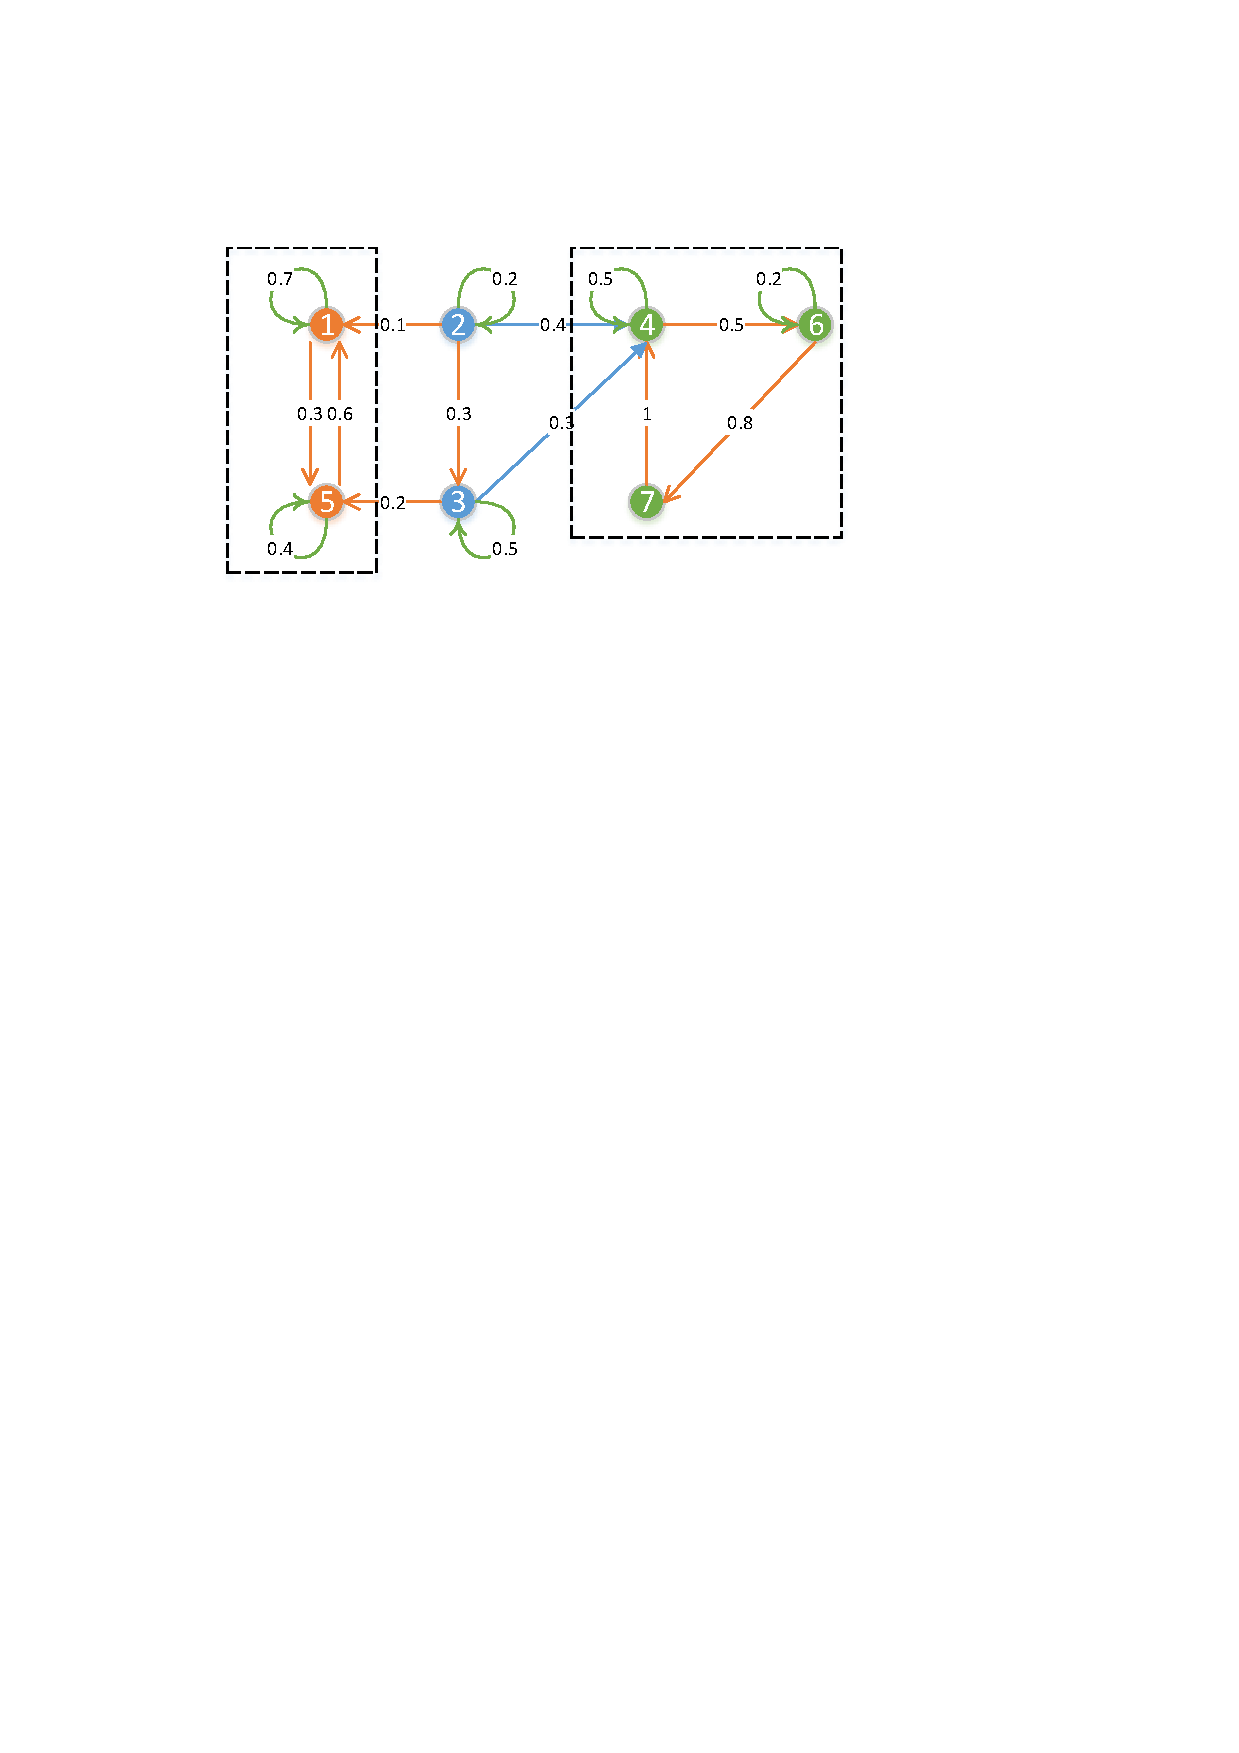
\includegraphics[scale=.6]{fig/markov2.pdf}
    \end{center}
    \begin{spacing}{1.2}
    \small
    状态2可达状态1、3和4;状态3可达状态5和4,但是从状态1、5、4、6、7却不可达状态2或3。这说明状态2和3是非常返态,即有正的概率不再返回原先的状态。

    相比之下,状态1和5,以及状态4、6、7分别组成的环状区域,可以实现状态的互通,状态互通意味着可以概率1返回原来的状态,因此状态1、5、4、6、7是常返态。
    \end{spacing}
\end{frame}

\subsection{状态空间的分解}
\begin{frame}{闭集的概念}
    若$x\in A$,并且$y\notin A$,则$p(x,y)=0$,称集合$A$是闭集(closed set)。所谓的闭集,就意味着$A$内部的状态无法到达$A$的外部,这意味着一旦状态进入闭集$A$中,它将永远留在其中运动。
    \begin{center}
		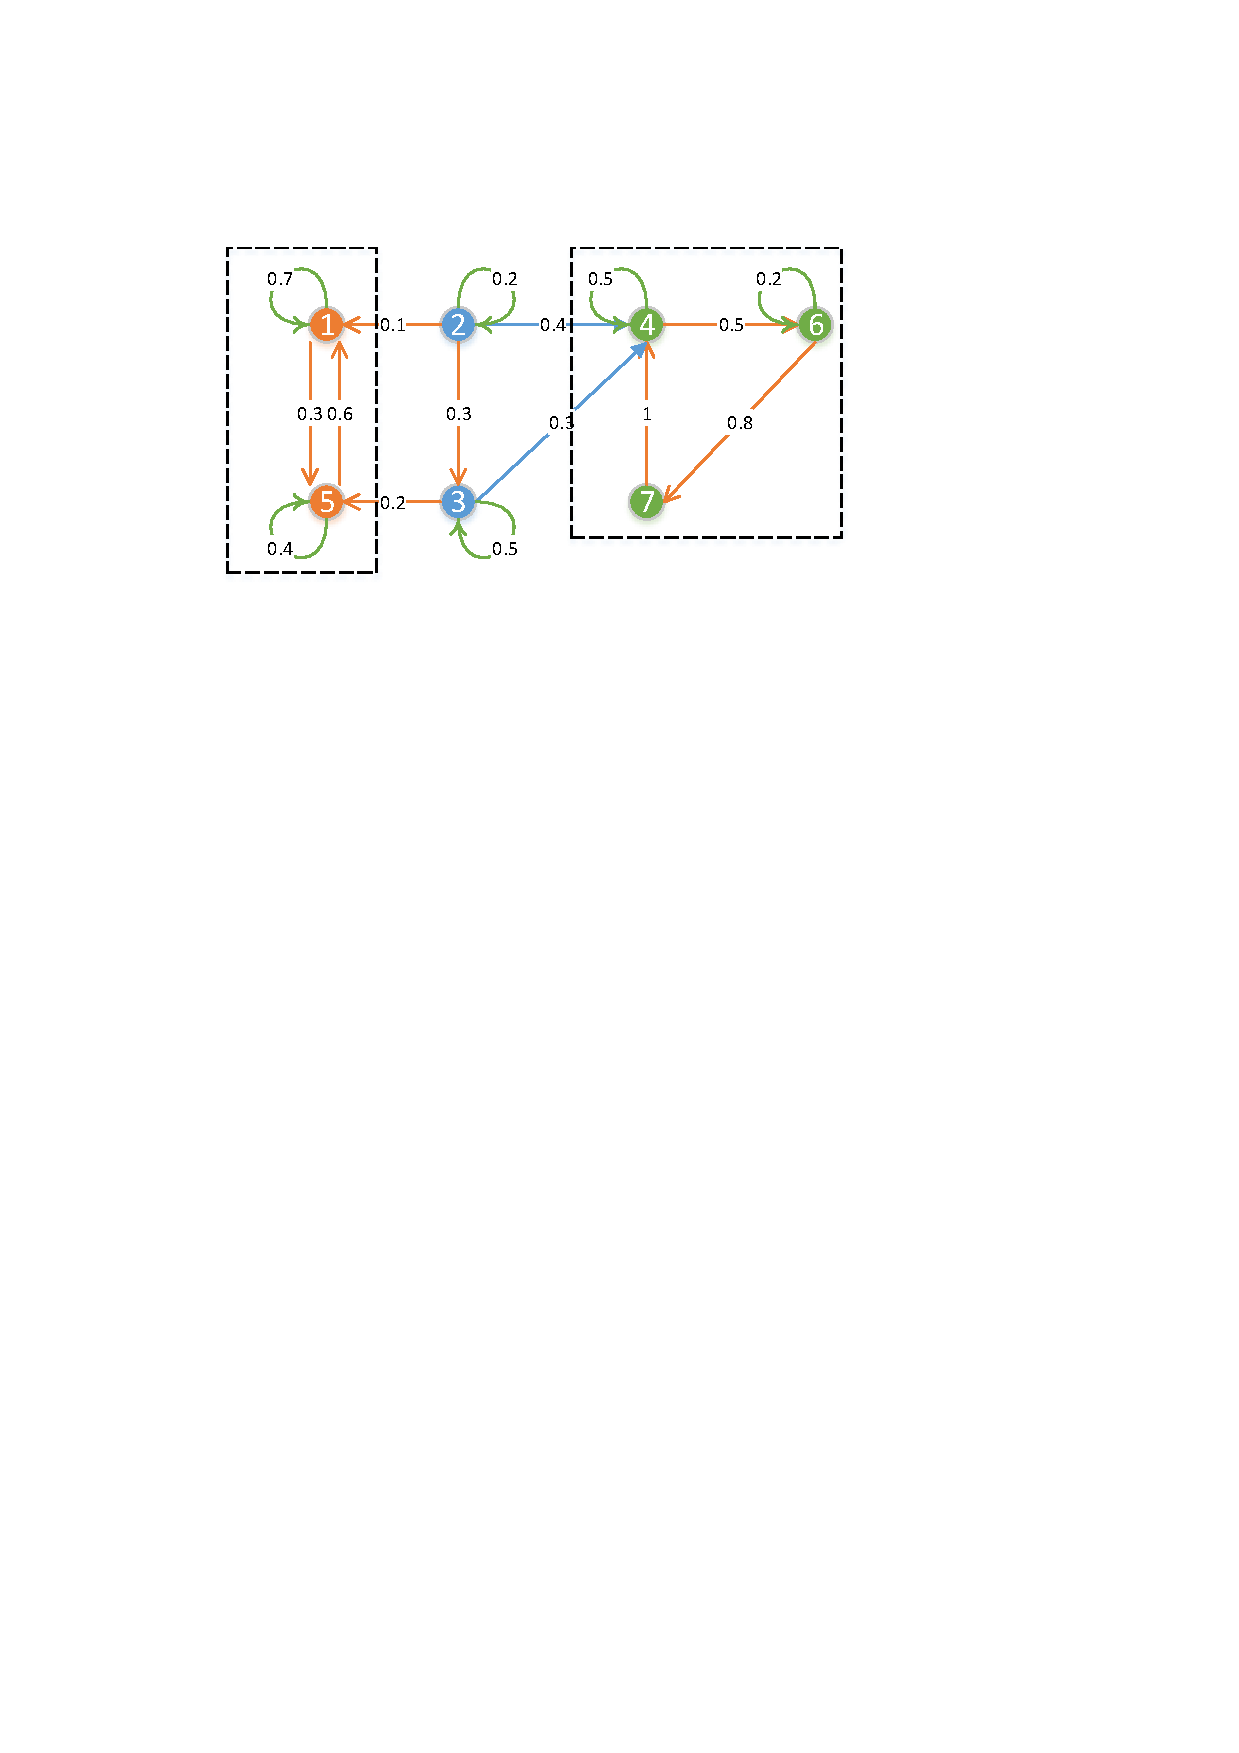
\includegraphics[scale=.5]{fig/markov2.pdf}
    \end{center}

    七状态马氏链中,状态1和5无法转移到其他状态;状态4、6、7也无法转移到其他状态,因此$\{1,5\}$和$\{4,6,7\}$是两个闭集。
\end{frame}


\begin{frame}{闭集的概念(cont.)}
更一般地,$\{1,5\}$和$\{4,6,7\}$的并集$\{1,4,5,6,7\}$也是闭集;整个状态空间$S=\{1,2,3,4,5,6,7\}$也必然是一个闭集,因为所有的状态转移均不可能超出这个状态空间。

\begin{block}{注意:}
    闭集的概念是普适的,只是前面例子中可以举出的闭集当中,有些闭集的元素太多,因此有必要对这些闭集进行限定,于是要引入不可约闭集的概念。
\end{block}
\end{frame}

\begin{frame}{不可约闭集}
    对于闭集$A$,若其中任意状态$x$和$y$均互通,则称闭集$A$是不可约闭集(irreducible closed set)。即:
    \[\forall x,y\in A,\quad x\leftrightarrow y \quad \Rightarrow\quad \text{$A$不可约}\]
    不可约闭集中的元素构成一个互通类。

    如果马氏链只有一个互通类,则称这个链不可约(irreducible);若互通类超过一个,则称这个链可约(reducible)。

    \begin{block}{}
        七状态马氏链中,$1\leftrightarrow 5$,并且$4\leftrightarrow 6\leftrightarrow 7$,因此$\{1,5\}$和$\{4,6,7\}$是两个不可约闭集。另外,这个马氏链包含了两个互通类,因此这是可约马氏链。
    \end{block}
\end{frame}

\begin{frame}{若干定理}
\begin{itemize}
    \item 对于任何互通类$C$而言,其中的所有状态均为常返态或非常返态。
    \item 对于一个有限闭集$C$,其中至少有一个常返态。
\end{itemize}
\end{frame}



\begin{frame}{状态空间的分解}
    若状态空间$S$是有限的(finite state space),则$S$可以写为互不相交集合的并集,即:
	\[S=T\cup R_1\cup \cdots \cup R_k \]
	其中,$T$是非常返态组成的集合;$R_i,\; i=1,2,\ldots,k$是常返态组成的不可约闭集。
\end{frame}


\begin{frame}{七状态马氏链回顾}
    \begin{spacing}{1.2}
   \small 对七状态马氏链的不可约闭集进行归并和整理,可得如下转移概率矩阵:
    \[\left[\begin{array}{cc|ccc|cc}
        0.7&0.3&0&0&0&0&0\\
        0.6&0.4&0&0&0&0&0\\
        \hline
        0&0&0.5&0.5&0&0&0\\
        0&0&0&0.2&0.8&0&0\\
        0&0&1&0&0&0&0\\
    \hline
        0.1&0&0.4&0&0&0.2&0.3\\
        0&0.2&0.3&0&0&0&0.5\\
    \end{array}
        \right]=\left[\begin{array}{c|c|c}
            {\bf R}_1 & \bf{0} &\bf{0}\\
            \hline
            \bf{0} &{\bf R}_2 &\bf{0}\\
            \hline
            {\bf T}_1 & {\bf T}_2 & {\bf T}
        \end{array}
            \right]
    \]
    其中,分块矩阵${\bf R}_1$和${\bf R}_2$分别由不可约闭集$\{1,5\}$和$\{4,6,7\}$构成,相应的状态均为常返态; 
分块矩阵${\bf T}$则是由非常返态$\{2,3\}$构成;分块矩阵${\bf T}_1$和${\bf T}_2$反映了由非常返态经过一步转移到常返态的对应转移概率。

两个由常返态所构成的不可约闭集之间的转移概率均为零,这也从侧面验证了不可约闭集的特点——其内的状态无法转移到闭集之外。
    \end{spacing}
\end{frame}


\begin{frame}{举例}
    设$S=\{1,2,\ldots,6\}$,相应的转移概率矩阵为:
    \[{\bf P}=\begin{bmatrix}
    0 & 0 & 1 & 0 & 0 & 0\\
    0 & 0 & 0 & 0 & 0 & 1\\
    0 & 0 & 0 & 0 & 1 & 0\\
    \frac{1}{3} & \frac{1}{3} & 0 & \frac{1}{3} & 0 & 0\\
    1 & 0 & 0 & 0 & 0 & 0\\
    0 & \frac{1}{2} & 0 & 0 & 0 & \frac{1}{2}
    \end{bmatrix} \]
    试分解此马氏链,并指出各状态的常返性。
\end{frame}


\begin{frame}{转移概率图}
	\begin{center}
		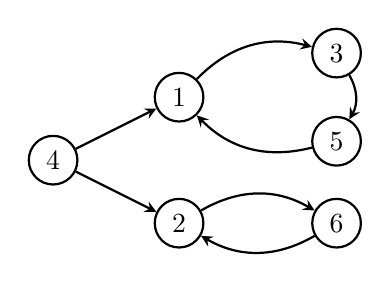
\begin{tikzpicture}[>=stealth, thick,scale=.8]
		\node [circle, draw] (A) at (0,0) {1};
		\node [circle, draw] (C) at (2.5,.7) {3};
		\node [circle, draw] (E) at (2.5,-.7) {5};
		\node [circle, draw] (B) at (0,-2) {2};
		\node [circle, draw] (F) at (2.5,-2) {6};
		\node [circle, draw] (D) at (-2,-1) {4};
		
		\draw[->] (A) to [bend left=30] (C);
		\draw[->] (E) to [bend left=30] (A) ;
		\draw[->] (F) to [bend left=30] (B);
		\draw[->] (B) to [bend left=30] (F);
		\draw[->] (D) to   (B);
		\draw[->] (D) to   (A);
		\draw[->] (C) to [bend left=30] (E);
		\end{tikzpicture}
        \end{center}
        
        $1\leftrightarrow 3\leftrightarrow 5$,$2\leftrightarrow 6$
。因此该马氏链当中,$\{1,3,5\}$和$\{2,6\}$分别构成一个互通类,且其中的各状态均为常返态;而$4\to 1,\; 4\to2$,故$\{4\}$是非常返态。

因此,该马氏链可以分解为两个由常返态组成的不可约闭集$\{1,3,5\}$和$\{2,6\}$,以及一个由非常返态构成的集合$\{4\}$。 
\end{frame}


\subsection{状态的周期}
\begin{frame}{周期的概念}
    一个状态$x$的周期是$I_x=\{n\ge 1:p^n(x,x)>0 \}$的最大公约数(greatest common divisor, gcd),记作
    \[d(x)={\rm gcd}\{n\ge 1:p^n(x,x)>0 \} \]
    若$d(x)>1$,则称状态$x$是周期的(periodic);若$d(x)=1$,则称状态$x$是非周期的(aperiodic)。

\end{frame}

\begin{frame}{周期的概念(cont.)}
    对于状态$x$而言,若其周期为$d(x)$,则根据定义,其回到原状态的步数$n$一定是$d(x)$的整数倍。

 \begin{block}{定理}
    $I_x$是加法封闭集(对加法运算封闭),即:若$m,\;n\in I_x$,则$(m+n)\in I_x$。
 \end{block} 
\end{frame}


\begin{frame}{举例6:三角形和正方形}
\begin{center}
    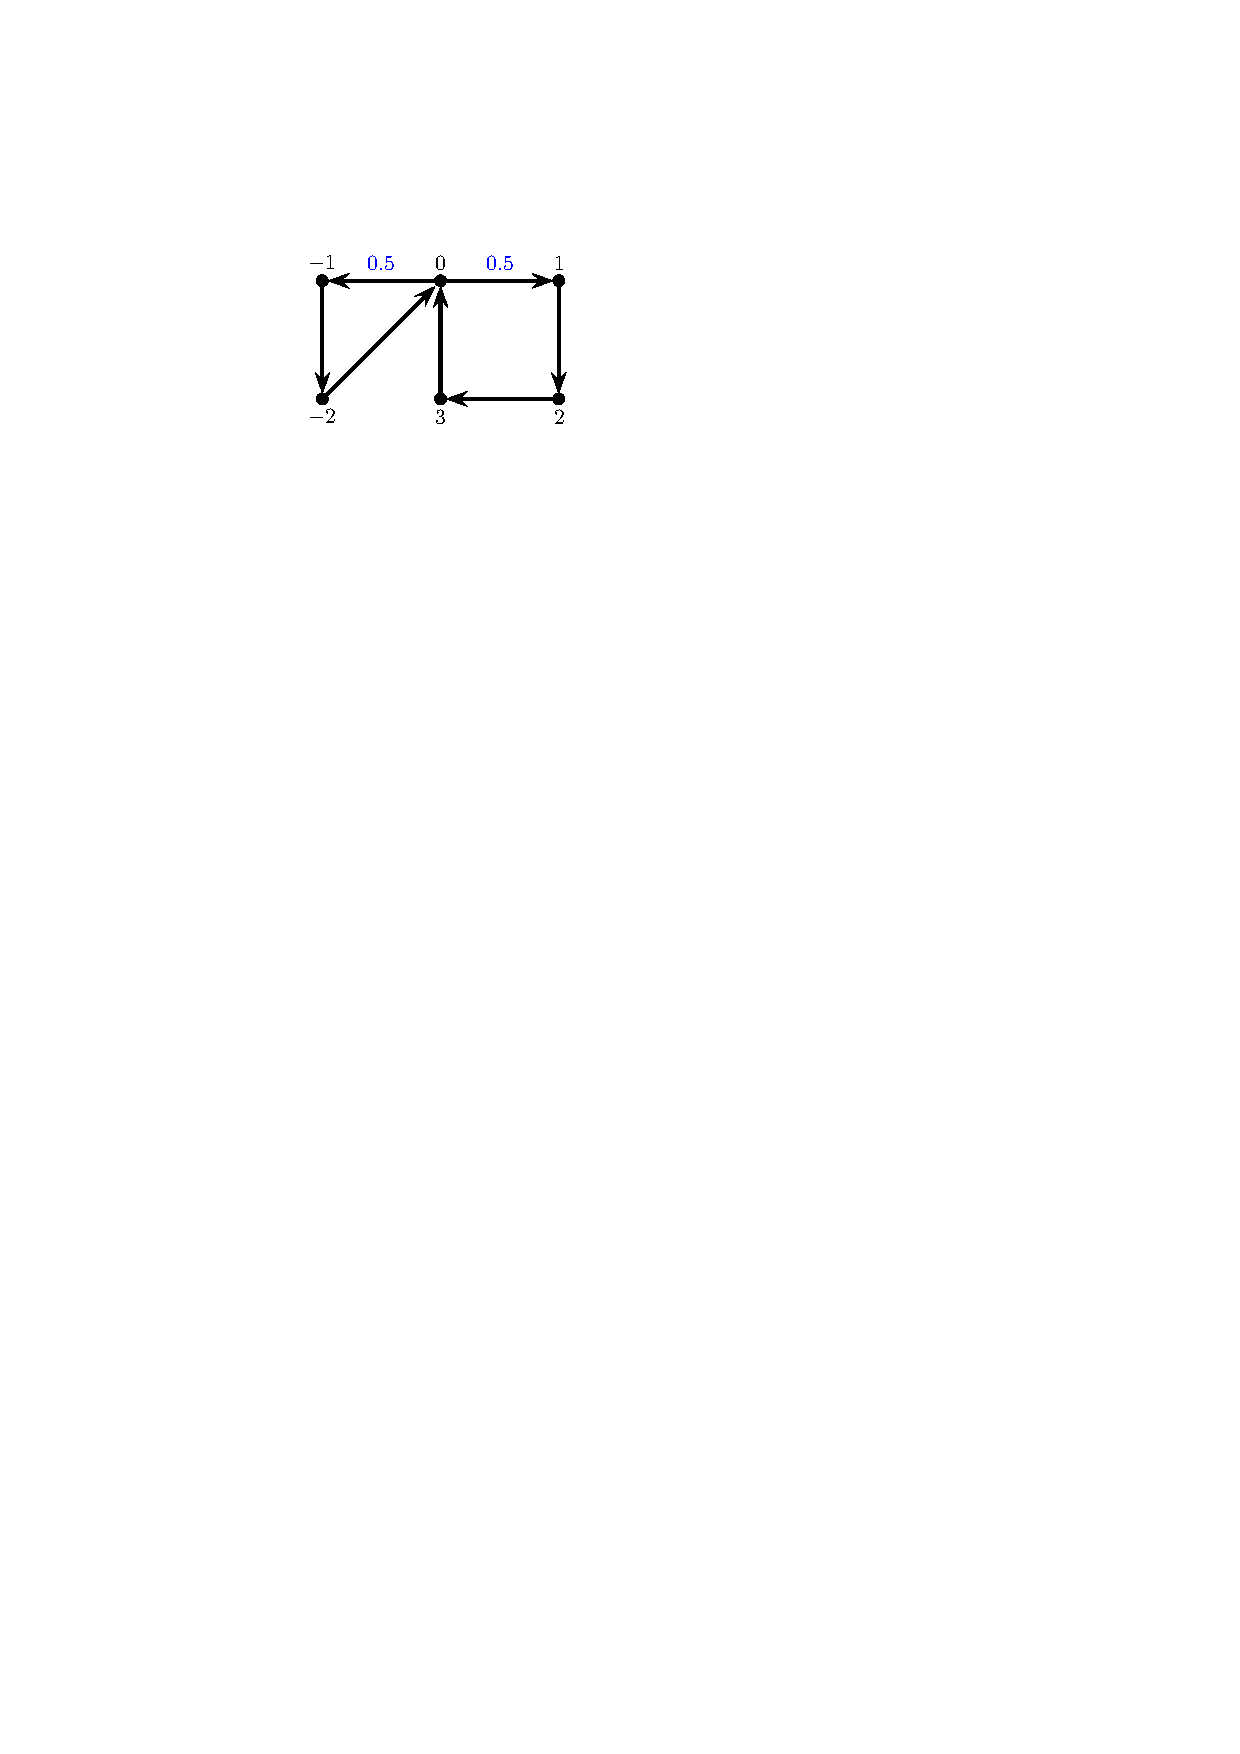
\includegraphics{fig/markov3.pdf}
\end{center}
状态0的左侧,$p^3(0,0)>0$;状态0的右侧,$p^4(0,0)>0$。因此:$3,4\in I_0$。由于$I_0$是加法封闭集,且$p^3(0,0)>0,\; p^4(0,0)>0$,因此:
\[I_0=\{3,4,6,7,8,9,10,11,12,\ldots\} \]
上面序列的最大公约数为1,所以状态0的周期为1。
\end{frame}


\begin{frame}{相关定理}
\begin{itemize}
    \item 若$p(x,x)>0$,则状态$x$的周期为1。
    \item 若$f_{xy}>0$,且$f_{yx}>0$,则状态$x$和$y$具有相同的周期。
\end{itemize}
\end{frame}


\begin{frame}{举例7:奇数个节点的环}
    \begin{center}
		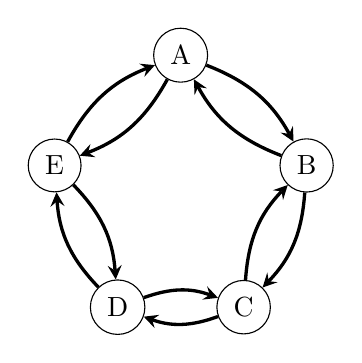
\begin{tikzpicture}[>=stealth,scale=.8]
		\node[draw,circle] (A) at (0,4) {A};
		\node[draw,circle] (B) at (2,2.25) {B};
		\node[draw,circle] (C) at (1,0){C};
		\node[draw,circle] (D) at (-1,0){D};
		\node[draw,circle] (E) at (-2,2.25){E};
		
		\draw[->, very thick](A)  to [bend left=20] (B);
		\draw[->, very thick](B)  to [bend left=20] (A);
		\draw[->, very thick](B)  to [bend left=20] (C);
		\draw[->, very thick](C)  to [bend left=20] (B);
		\draw[->, very thick](C)  to [bend left=20] (D);
		\draw[->, very thick](D)  to [bend left=20] (C);
		\draw[->, very thick](D)  to [bend left=20] (E);
		\draw[->, very thick](E)  to [bend left=20] (D);
		\draw[->, very thick](E)  to [bend left=20] (A);
		\draw[->, very thick](A)  to [bend left=20] (E);
        \end{tikzpicture}
    \end{center}
    
    以节点A为例,其沿顺时针方向遍历一圈,返回状态A的步数为5;A$\to$B$\to$A的步数为2。可见,$2,5\in I_A$,其最大公约数${\rm gcd}(2,5)=1$。因此,此时的周期为1,该马氏链{非周期}。
\end{frame}


\begin{frame}{举例8:偶数个节点的环}
        \begin{center}
        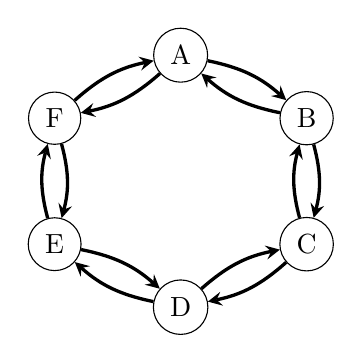
\begin{tikzpicture}[>=stealth,scale=.8]
            \node[draw,circle] (A) at (0,4) {A};
            \node[draw,circle] (B) at (2,3) {B};
            \node[draw,circle] (C) at (2,1){C};
            \node[draw,circle] (D) at (0,0){D};
            \node[draw,circle] (E) at (-2,1){E};
            \node[draw,circle] (F) at (-2,3){F};
            
            \draw[->, very thick](A)  to [bend left=15] (B);
            \draw[->, very thick](B)  to [bend left=15] (A);
            \draw[->, very thick](B)  to [bend left=15] (C);
            \draw[->, very thick](C)  to [bend left=15] (B);
            \draw[->, very thick](C)  to [bend left=15] (D);
            \draw[->, very thick](D)  to [bend left=15] (C);
            \draw[->, very thick](D)  to [bend left=15] (E);
            \draw[->, very thick](E)  to [bend left=15] (D);
            \draw[->, very thick](E)  to [bend left=15] (F);
            \draw[->, very thick](F)  to [bend left=15] (E);
            \draw[->, very thick](F)  to [bend left=15] (A);
            \draw[->, very thick](A)  to [bend left=15] (F);
            
            \end{tikzpicture}
    \end{center}
    
    以节点A为例,其沿顺时针方向遍历一圈,返回状态A的步数为6;A$\to$B$\to$A的步数为2。可见,$2,6\in  I_A$,其最大公约数${\rm gcd}(2,6)=2$。因此,该马氏链的{周期为2}。
\end{frame}

\begin{frame}{举例:}
    求以下马氏链的周期:
    \begin{center}
    ${\bf P}=$\begin{blockarray}{cccccc}
        & 1 & 2 &3	&4 & 5  \\	
            \begin{block}{c[ccccc]}
    1 &0&   0.3&  0.7&         0 &        0\\
    2   & 0&        0&         0&        $0.25$  &      $0.75$   \\
    3&0 &   0&         0   & $0.5$     &   $0.5$     \\
    4&1  &       0 &        0 &        0  &  0\\
    5&1   &      0  &       0  &       0      &   0\\
            \end{block} 
    \end{blockarray}
    \end{center}
\end{frame}

\begin{frame}{转移概率图}
        \begin{center}
            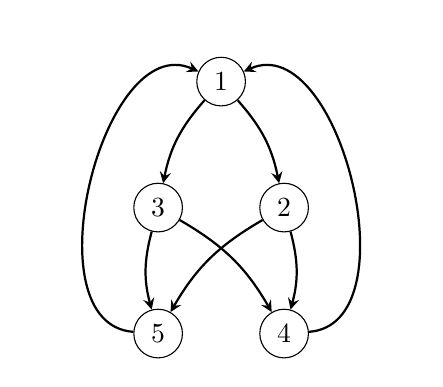
\begin{tikzpicture}[>=stealth,scale=.8]
            \node[draw,circle] (A) at (0,0) {1};
            \node[draw,circle] (B) at (1,-2) {2};
            \node[draw,circle] (C) at (-1,-2){3};
            \node[draw,circle] (D) at (1,-4){4};
            \node[draw,circle] (E) at (-1,-4){5};
            
            \draw[->, thick](A)  to [bend left=15] (B);
            \draw[->, thick](A)  to [bend left=-15] (C);
            \draw[->, thick](B)  to [bend left=15] (D);
            \draw[->, thick](B)  to [bend left=-15] (E);
            \draw[->, thick](C)  to [bend left=15] (D);
            \draw[->, thick](C)  to [bend left=-15] (E);
            \draw[->, thick](D)  to [bend left=-100] (A);
            \draw[->, thick](E)  to [bend left=100] (A);
            
            \end{tikzpicture}
            \end{center}

            以状态1为例,其再次访问原状态的路径有:$1\to 3\to5\to1$;$1\to 3\to4\to1$;$1\to 2\to5\to1$;$1\to 2\to4\to1$,各路径下的步数均为3,可见,$d(1)=3$。类似地,其他状态的周期也均为3。因此,该马氏链的周期为3。
\end{frame}


\end{document}